\documentclass[11pt,letterpaper,article,oneside]{memoir}
\usepackage[utf8]{inputenc}
\usepackage[T1]{fontenc}
\usepackage{microtype}
\usepackage[dvips]{graphicx}
\usepackage{xcolor}
\usepackage{times}

\usepackage{booktabs}

\usepackage{enumitem}
\setlist[description]{style=nextline}
\setlist[itemize]{nosep}

\usepackage[
breaklinks=true,colorlinks=true,
linkcolor=blue,urlcolor=blue,citecolor=blue,% PDF VIEW
%linkcolor=black,urlcolor=black,citecolor=black,% PRINT
bookmarks=true,bookmarksopenlevel=2]{hyperref}

\usepackage{geometry}
% PDF VIEW
% \geometry{total={210mm,297mm},
% left=25mm,right=25mm,%
% bindingoffset=0mm, top=25mm,bottom=25mm}
% PRINT
\geometry{total={210mm,297mm},
left=20mm,right=20mm,
bindingoffset=10mm, top=25mm,bottom=25mm}

\OnehalfSpacing

%%% STYLE OF SECTIONS, SUBSECTIONS, AND SUBSUBSECTIONS
\setsecheadstyle{\large\bfseries\raggedright}
\setsubsecheadstyle{\bfseries\raggedright}


%%% STYLE OF PAGES NUMBERING
\pagestyle{plain}
\makepagestyle{plain}
\makeevenfoot{plain}{\thepage}{}{}
\makeoddfoot{plain}{}{}{\thepage}
\makeevenhead{plain}{}{}{}
\makeoddhead{plain}{}{}{}

\maxsecnumdepth{section}
\maxtocdepth{section}



\newcommand{\name}{PROGRAM\_NAME}
\newcommand{\programVersion}{0.1}
\newcommand{\manualVersion}{0.1}
\newcommand{\email}{eric.tytell@tufts.edu}

\newcommand{\csv}{\texttt{.csv}}
\newcommand{\hdf}{\texttt{.hdf5}}


\renewcommand{\arraystretch}{1.2}

\setlength{\parindent}{0em}
\nonzeroparskip





\begin{document}

\thispagestyle{empty}

{%%%
\centering
\Large

\vspace*{\fill}

{\huge
\name{} \programVersion{}
}

{\LARGE
%User manual version \manualVersion{} \\
User manual \\
}
\vspace*{\fill}

}

\cleardoublepage

\tableofcontents*

\clearpage



%%%%%%%%%%%%%%%%%%%%%%%%%%%%%%%%%%%%%%%%%%%%%%
%                 LICENSE                    %
%%%%%%%%%%%%%%%%%%%%%%%%%%%%%%%%%%%%%%%%%%%%%%

\chapter{Copyright and License}

\name{}: a tool for collecting IMU measurements.
Copyright (C) 2017 \textbf{Authors???}/

This program is free software: you can redistribute it and/or modify
it under the terms of the GNU General Public License as published by
the Free Software Foundation, either version 3 of the License, or
(at your option) any later version.

This program is distributed in the hope that it will be useful,
but WITHOUT ANY WARRANTY; without even the implied warranty of
MERCHANTABILITY or FITNESS FOR A PARTICULAR PURPOSE.  See the
GNU General Public License for more details.

You should have received a copy of the GNU General Public License
along with this program.  If not, see \url{http://www.gnu.org/licenses/}.



%%%%%%%%%%%%%%%%%%%%%%%%%%%%%%%%%%%%%%%%%%%%%%
%               INTRODUCTION                 %
%%%%%%%%%%%%%%%%%%%%%%%%%%%%%%%%%%%%%%%%%%%%%%

\chapter{Introduction}

\name{} is an application for recording and processing data from inertial
measurement units (IMUs). It consists of two parts. Microcontroller code running
on an Arduino board collects data from the IMUs and transmits it to a PC. A
Python program running on the PC receives data from the Arduino and provides
users with a graphical interface. This interface allows users to interact with
the Arduino and to view and manipulate IMU data.



%%%%%%%%%%%%%%%%%%%%%%%%%%%%%%%%%%%%%%%%%%%%%%
%             SECTION: HARDWARE              %
%%%%%%%%%%%%%%%%%%%%%%%%%%%%%%%%%%%%%%%%%%%%%%

\chapter{Hardware}

\name{} interconnects three pieces of computational hardware: a PC, an Arduino,
between 1 and 3 IMUs.

\section{PC}
\name{} has been tested on PCs running Linux Mint 18 Sarah, OS X El Capitan
10.11, and Windows 10. It is expected to work with other versions of these
operating systems and with other Linux distributions.

\section{Arduino}
\name{} has been tested with an Arduino UNO. It may work on other
models with a 16MHz clock speed and sufficient storage.


\section{IMUs}
The mpu9250 by InvenSense is a nine-axis (gyroscope, accelerometer, compass)
motion tracking device.

For applications requiring minimum package size and weight,
the mpu9250 can be wired directly to the Arduino. A separate manual
documents the procedure we have used to prepare the mpu9250 for use with
\name{}:
\url{http://www.url_for_cassandras_manual.com}

For testing purposes, or if the added size and weight are acceptable, an mpu9250
mounted on a circuit-board can be used with \name{}.


\section{SPI}
The Arduino communicates with the IMUs using the Serial Peripheral Interface bus
(SPI) protocol. With SPI, one or more slave devices (IMUs in this application)
exchange data with a master device (the Arduino) over a single shared bus,
consisting of 2 data lines and a clock line. Each slave has a separate
\emph{chip select} line, used to control access to the shared bus.

\section{Wiring the Arduino}
\label{sec:wiring}
Table \ref{tab:wiring} summarizes the process of connecting IMUs to the Arduino.
It may be necessary to use a breadboard, especially if multiple IMUs are used.
Figure \ref{fig:wiring} shows an Arduino wired to a single IMU.  Pins 8, 9, and
10 are used for \emph{chip select} lines for up to three IMUs. Pin 11 carries
data traveling from the Arduino to the IMUs, i.e. Master-Out, Slave-In (MOSI).
Pin 12 carries data traveling from the IMUs to the Arduino, i.e. Master-In,
Slave Out (MISO). Pin 13 carries a clock signal which regulates timing of the
communication protocol.  Each IMU should be connected to 3.3V power (available
on the Arduino) and to ground.

If using a trigger, connect it to Pin 4 and to ground.

Connect the Arduino to the PC with a USB cable.  To ensure adequate power,
especially if using multiple IMUs, it is recommended to power the Arduino with
an external power source instead of relying on the USB port.

\begin{table}
\centering
\begin{tabular}{@{}*4l@{}}
\toprule
description & label & color & pin \\
\midrule 
IMU 1 chip select & NCS / CS & white & 8 \\
IMU 2 chip select & NCS / CS & white & 9 \\
IMU 3 chip select & NCS / CS & white & 10 \\
data from Arduino to IMU & MOSI / SDA & green & 11 \\
data from IMU to Arduino & MISO / SDO & blue & 12 \\
clock & SCL / CLK & yellow & 13 \\
power &  & red & 3.3V \\
ground &  & black & GND \\
trigger &  &  & 4 \\
\bottomrule
\end{tabular}
\caption{Instructions for wiring the IMUs to the Arduino. The first column
describes the purpose of each line. The second column provides names commonly
used to describe each line. For example, if the IMU is mounted on a board, the
board's pins might have labels matching these values. The third column provides
the colors specified in the \textbf{Document Name} manual. The fourth column
specifies pins on the Arduino Uno.}
\label{tab:wiring}
\end{table}

\begin{figure}[]
    \begin{center}
        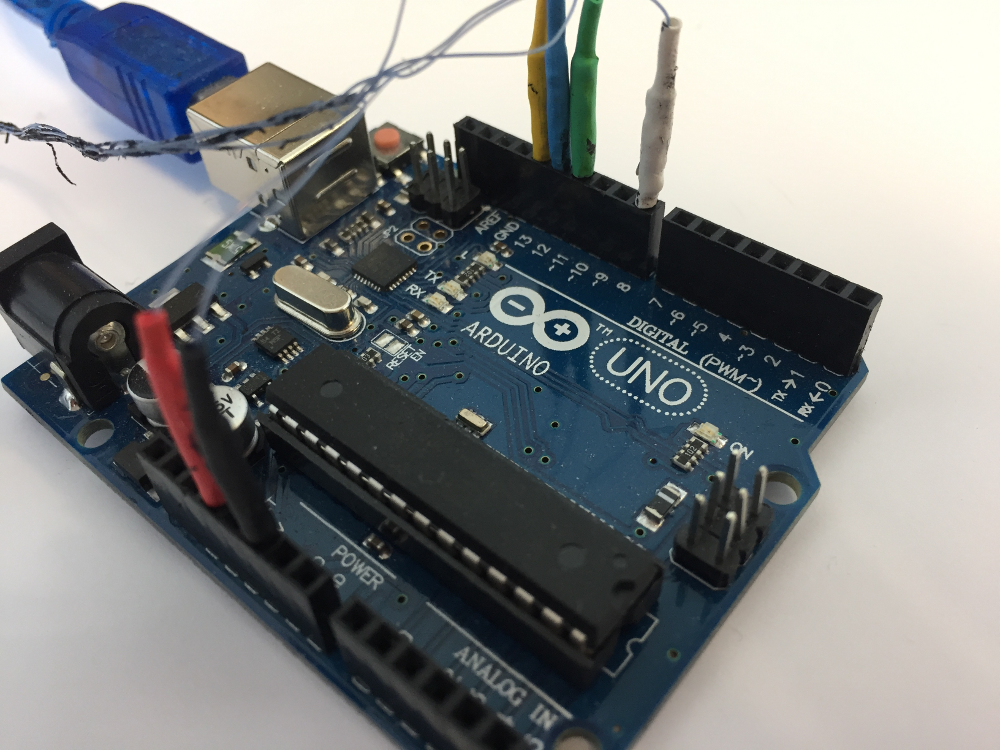
\includegraphics[height=3in]{wiring}
    \end{center}
    \label{fig:wiring}
    \caption{Wiring a single IMU to the Arduino}
\end{figure}



%%%%%%%%%%%%%%%%%%%%%%%%%%%%%%%%%%%%%%%%%%%%%%
%          SECTION: INSTALLATION             %
%%%%%%%%%%%%%%%%%%%%%%%%%%%%%%%%%%%%%%%%%%%%%%

\chapter{Installation}

\section{Arduino IDE}
While there are many tools for installing program code onto the Arduino, we have
tested \name{} using the Arduino IDE version 1.8.1.
Earlier versions might lack some of library definitions used by \name{}.

The software can be downloaded from:
\url{https://www.arduino.cc/en/Main/Software}

If your operating system has a package management system, it might be able
to install the Arduino IDE. For example, on a Debian-based system you can use
\texttt{apt}:
\begin{verbatim}
# apt install Arduino-core
\end{verbatim}

\section{Install \name{} on the Arduino}
\label{sec:installarduinocode}

Transfer the file \verb|am_tx/am_tx.ino| onto Arduino.  This can be accomplished
using the Arduino IDE graphical user interface.  Alternatively, the Arduino IDE
can be used to program the Arduino directly from the command line:

\begin{verbatim}
# arduino --upload am_tx/am_tx.ino
\end{verbatim}

For more information about the Arduino command line interface, see:
\url{https://github.com/arduino/Arduino/blob/master/build/shared/manpage.adoc}

\section{PC}
\label{sec:installPc}
\name{} requires Python 3. It has been tested with Python version 3.5. Thus, it
is recommended to use Python version 3.5 or later.

Consider using \texttt{virtualenv} to isolate your installation of \name{} from
other packages and from other Python versions:
\url{https://pypi.python.org/pypi/virtualenv}

We recommend using pip to install \name{}:
\url{https://pypi.python.org/pypi/pip}

\begin{verbatim}
# cd PROGRAM_NAME
# pip install --upgrade pip
# pip install ./
\end{verbatim}

Pip will automatically install any of the following dependencies if needed:
\begin{itemize}
\item h5py
\item numpy
\item pyqtgraph
\item pyserial
\item pyqt5
\end{itemize}

Once \name{} has been installed, it can be started from the command line:\\
\texttt{
\# \name{}
}

\begin{figure}[]
    \begin{center}
        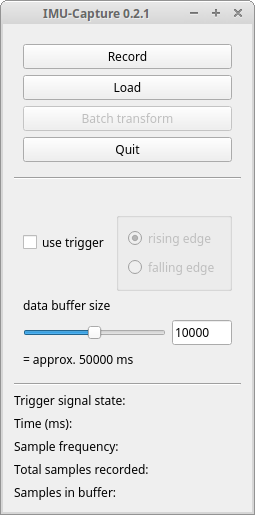
\includegraphics[height=3in]{screenshot_panel}
    \end{center}
    \caption{Control panel} 
\end{figure}


\chapter{The data buffer}
\name{} uses a single data buffer to hold IMU data. When data is recorded from
the IMUs, the data buffer is first erased. Then each sample is added to the
buffer as it is recorded. The buffer can be saved to a file, or a file can be
loaded into the buffer, erasing any previous contents. Data processing
operations can be performed on the data buffer, altering it irreversibly.
Therefore, any time the data buffer contains valuable data it is recommended to
save it to file before collecting new data, loading another file, or executing
data processing operations.

The \emph{data buffer length (\# samples)} slider adjusts the size of the data
buffer. When each new sample is received, it is added to the data buffer. If the
buffer was already full (the number of samples in the buffer was equal to the
size of the buffer), the oldest sample in the buffer is deleted. If the size of
the buffer is adjust to be smaller than the number of samples in the buffer, the
oldest samples in the buffer are deleted until the number of samples in the
buffer is equal to the buffer length.


\chapter{Collecting data}

To begin collecting data, press the \emph{record} button.  The \emph{record} button
changes into the \emph{stop} button.  The PC establishes communication with to the
Arduino and instructs it to begin collecting data from the IMUs at 200Hz. This
sample rate is hard-coded, and was determined to be near the maximum possible
with the Arduino Uno.

As samples received from the Arduino are recorded in the data buffer, they
become visible in the data visualization plots. For each IMU, one row of three
plots is displayed. The left-most plot shows accelerometer data, the center plot
shows gyroscope data, and the right-most plot shows magnetometer data. For each
plot, red, green, and blue lines show x, y, and z axis measurements,
respectively.

The \emph{stop} button (or the trigger, as described in Section \ref{sec:trigger}),
causes the PC first to instruct the Arduino to stop collecting data and then to
halt communication with the Arduino. The \emph{stop} button changes back into the
\emph{record} button.

\begin{figure}[]
    \begin{center}
        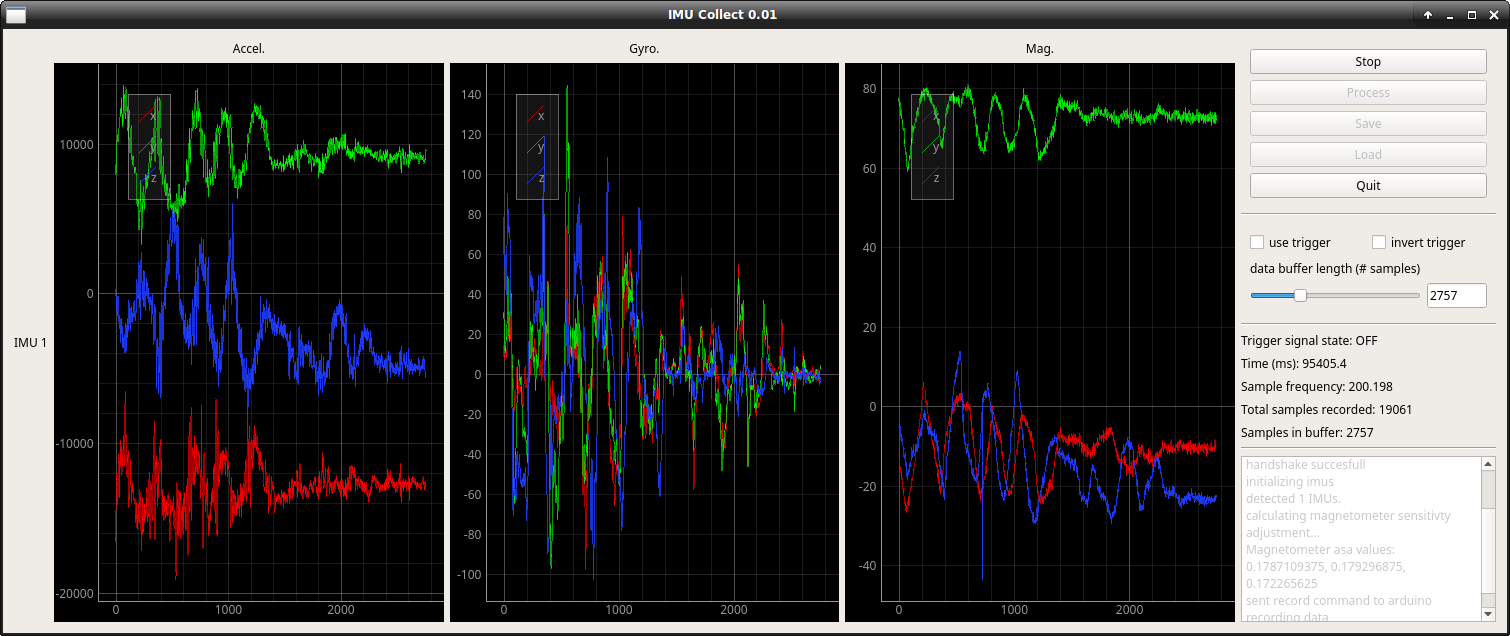
\includegraphics[width=\textwidth]{screenshot_plots}
    \end{center}
    \caption{Collecting data from a single IMU} 
\end{figure}



\section{Trigger}
\label{sec:trigger}

Optionally, a trigger attached to the Arduino (Section \ref{sec:wiring}) can be
used to stop recording.  If the \emph{use trigger} checkbox is not checked, the
trigger is ignored. Otherwise, if an active trigger is detected, recording will
stop, i.e., the same effect as pressing the \emph{stop} button during recording.
If the \emph{Record} is pressed while the \emph{use trigger} checkbox is checked
and the trigger is active, the recording immediately ends with zero data stored.

If the \emph{invert trigger} checkbox is not checked, the trigger is considered
active when the associated Arduino pin is set high. If the \emph{invert trigger}
checkbox is checked, the trigger is considered active when the associated
Arduino pin is set low.

If no trigger is connected then the value of the pin is undefined.  Thus, to
ensure reliable behavior, the \emph{use trigger} checkbox should not be checked
unless there is a trigger connected to the Arduino.



\chapter{Saving and loading}
\label{sec:savingloading}

\section{File formats}

\label{sec:fileformats}
The \csv{} file format stores data in plain text, using newlines to delimit
samples and commas to delimit measurements within each sample.  \name{} uses the
CSV module in the Python Standard Library with default formatting parameters:
\url{https://docs.python.org/3/library/csv.html}

The \hdf{} format is designed to store large amounts of data. It is generally more
compact than \csv{}. \name{} uses the h5py package to read and write \hdf{} files:
\url{http://www.h5py.org/}


\section{Saving}

The \emph{save} button opens a dialog allowing the user to select a filesystem
location, a filename, and a filetype (either \csv{} or \hdf{}).  The the data
buffer is saved to file according to the selections made in the dialog. The
\emph{save} button is disabled when the data buffer is empty or while data is
being recorded.

\section{Loading}

The \emph{load} button opens a dialog allowing the user to select a filetype
(either \csv{} or \hdf{}) and a file to load. The file will be loaded into the
data buffer, overwriting any data stored there.  The \emph{load} button is
disabled while data is being recorded.


\chapter{Processing data}

\begin{figure}[]
    \begin{center}
        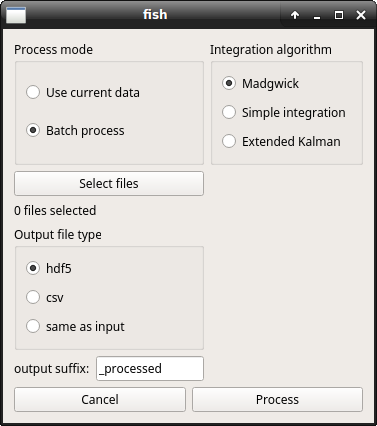
\includegraphics[height=3in]{screenshot_process}
    \end{center}
    \caption{Data processing control panel} 
    \label{fig:control}
\end{figure}

The \emph{process} button opens the data processing control panel (Figure
\ref{fig:control}).

\section{Process mode}
All data transformation algorithms are applied to the data buffer. If the \emph{Use
current data} radio button is selected, the current contents of the data buffer
are used. This option is not available when the data buffer is empty.

Alternatively, if the \emph{Batch process} radio button is selected, the current
contents of the data buffer are ignored. Instead, batch processing iterates over
a list of one or more input files, loading each file into the data buffer,
applying a transformation algorithm, and saving the result to a new output file
before proceeding to the next input file in the list. The \emph{Select files}
button launches a dialog for selecting input files for batch processing.  The
batch processing output filetype can be set, or can vary to match the filetype
of each input file. The output suffix string is appended to the filename of each
input file (before the file extension) to compose the output filename. If the
output suffix string is empty and the output filetype matches the input
filetype, then the input file is overwritten.

With either processing mode, the contents of the data buffer are overwritten by
any data processing.

\section{Integration algorithm}

The \emph{Integration algorithm} radio buttons select the data transformation
algorithm.

\begin{description}

\item[Madgwick]
We need to write about what this does.
\item[Simple integration]
We need to write about what this does.
\item[Extended Kalman]
We need to write about what this does.

\end{description}





\chapter{Troubleshooting}

\section{Installation}

If you encounter problems during installation, make sure you are using Python
3.5 or later and that pip is working with the correct Python version. Consider
using \texttt{virtualenv} as discussed in Section \ref{sec:installPc}.


\section{Error messages}

\newcommand{\genericFix}{Try resetting the Arduino.  Make sure that the Arduino
is correctly powered and connected to the PC (Section \ref{sec:wiring}), and
that the correct code is installed on the Arduino (Section
\ref{sec:installarduinocode}).}

This section provides explanation and troubleshooting tips for each error
message produced by \name{}. Error messages are printed in red type in the main
text window.

\begin{description}

\item[ASA read failed, using 1 adjustment]
For each magnetometer axis, a sensitivity adjustment value (ASA) is stored in
ROM by the manufacturer.  This error message is reported when the Arduino is
unable to read the ASA values from an IMU.  It likely indicates that the Arduino
is not communicating correctly with the magnetometer.  Any magnetometer data
recorded despite this message should be discarded.
\genericFix{}

\item[failed to create connection, aborting]
The program failed to establish a serial connection with the Arduino.
\genericFix{}

\item[handshake failed]
Even though the PC may have established a valid serial connection to the
Arduino, the data exchange protocol used by \name{} failed to establish a
communication handshake with the Arduino.
\genericFix{}

\item[invalid csv file]
The program attempted to read a .csv file (Section \ref{sec:fileformats}), but
the format of the data in the file was not valid.

\item[invalid file type:\ldots]
There was an attempt either to save or to load a filetype other than
\csv{} and \hdf{}. As discussed in Section \ref{sec:fileformats},
\csv{} and \hdf{} are the only file formats supported by \name.

\item[no Arduino found]
The program searched for Arduinos on all serial ports but didn't find any.
\name{} uses \texttt{serial.tools.list\_ports} to scan for Arduinos:
\url{http://pyserial.readthedocs.io/en/latest/tools.html}

\item[no IMUs detected, aborting]
The Arduino did not detect any attached IMUs.  After the Arduino is initialized,
it attempts to determine the number of IMUs by sending a WHOAMI request while
signaling each of the three legal chip select pins (Section \ref{sec:wiring}).
It then sends a message to the PC reporting the number of responses received. This
error is reported if the Arduino does not receive any WHOAMI responses.
\genericFix{}

\item[rx failed, no data read from serial]
The PC expected to receive data from the Arduino but failed. Perhaps no data was
transmitted, or perhaps only data that violates the communication protocol used
by \name{} was received.
\genericFix{}

\item[unknown sample received:\dots]
The PC expected to receive a packet containing a data sample, but the packet
either had the wrong type or the wrong length. This message can be ignored if it
occurs only briefly at the beginning of recording. Otherwise, try resetting the
Arduino.

\item[unable to determine number of IMUs, aborting]
The program failed to determine how many IMUs are attached to the Arduino. After
the Arduino is initialized, it attempts to determine the number of IMUs by
sending a WHOAMI request while signaling each of the three legal chip select
lines (Section \ref{sec:wiring}). It then sends a message to the PC reporting the
number of IMUs detected. This error is reported if the PC sends a
command to the Arduino to initialize, but does not receive a message reporting
the number of IMUs detected.
\genericFix{}


\end{description}




\end{document}

